\documentclass{article}
\usepackage{amsmath}
\usepackage{amssymb}
\usepackage{algorithm}
\usepackage{float}
\usepackage{color}
\usepackage{multicol}
\usepackage{forloop}
\usepackage{graphicx}
\usepackage[margin=0.8in]{geometry}
\usepackage{caption}
\graphicspath{ {./} }
\title{Neural Networks Final Project: \\
	\large{Comparing different data pre-processing techniques for convolution neural networks}}
\author{Krystian Wojcicki, 101001444 \\ Michael Kuang, 101000485}
\date{COMP 4107, Fall 2018}

\begin{document}
\maketitle

%Define figure width
\newcommand{\figureWidth}{0.25}
\section{Introduction}
\paragraph{}
{\em Natural Images} is a dataset currently featured on {\em kaggle.com}. The set is comprised of 6899 images from 8 distinct classes of airplane, car, cat, dog, flower, fruit, motorbike and person. Each class has a varying number of examples. We examined different techniques in pre-processing images and implemented them to analyze their effects on performance in a convolution neural network. 

\section{Problem Statement}
\paragraph{}
This project attempts to address the problems: "Do different image resizing techniques make a difference to classification accuracy?" and "Do balanced datasets improve classification accuracy?".

\section{Background}
\paragraph{}
One problem we looked at is the Class Imbalance problem, and this is the problem in machine learning where we have great discrepancy in the number of examples between class data. In other words, there are far more examples of one class than another in a set of data. This is a problem because as we know, machine learning works best when we have a more uniform distribution of data. In this project, we examine the performance between two up-sampling techniques called Synthetic Minority Over sampling Technique (SMOTE) and ADAptive SYNthetic (ADASYN) as solutions to class imbalance. 
\par
Another problem we investigated is how image resizing can affect performance. Given a set of non-uniform sizes of images, we must resize them to some constant shape in order to feed examples into the network. We examined two methods; resize the image by scaling it, and crop or pad the image about the center. The problem with resizing an image is that we inevitably lose information as images are scaled down or add noise as they are scaled up, but we are able to retain the information more uniformly. Cropping the image will directly lose the information as we resize the image by cropping out the outer most part of the image, while padding the image with black pixels evenly about center will retain the image aspect ratio.

\subsection{The Dataset}
\paragraph{}
The {\em Natural Images} dataset contains 6899 distinct RGB images of varying sizes for 8 classes as described below:
\begin{multicols}{2}

\begin{itemize}
	\item airplane: 727 
	\item car: 968
	\item cat: 885
	\item dog: 702
	\item flower: 843
	\item fruit: 1000
	\item motorbike: 788
	\item person: 986
\end{itemize} 

\end{multicols}
\subsection{Machine Learning Libraries}
\paragraph{}
Four libraries were used to implement our code, and create our neural network model: Tensorflow, scikit-learn, imbalanced-learn and OpenCV.

\subsection{Methodology}

\subsubsection{Scaling vs Crop and Pad}
\paragraph{}
We used OpenCV's resize method to scale the images down to or up to a specified size using nearest neighbour interpolation. The nearest neighbour interpolation is a point sampling algorithm that, rather than calculate the average or some weighting criteria, simply determines the nearest neighbouring pixel and assumes the intensity value of it. Using this method, it will upscale or downscale to a specified size. This method will add noise when we upscale or lose information when we downscale, and it is noted that the image will lose its original aspect ratio.
\par
Resizing an image by crop and pad means that the image will retain it's image resolution, but we either crop or pad the image about the center to the specified size. So, if the height of the image needs to be smaller, we crop the top and bottom evenly. Conversely, if the height of the image needs to be larger, we evenly pad the top and bottom with black pixels.	

To crop images, we simply used Python's built in array slicing on numpy arrays. Then, to pad or resize images, we used the following methods from the OpenCV library:
\begin{itemize}
	\item cv2.copyMakeBorder: padded the borders of the image by a specified amount using pixel color value of 0
	\item cv2.resize: resizes a given image to a specified height and width using interpolation method INTER\_NEAREST
\end{itemize}


\subsubsection{Spatial Pyramid Pooling}
\paragraph{}
CNNs require a fixed input image size such as 32x32, 64x64 or 128x128 as experimented with in this report. This requirement is human made and artificial while also potentially decreasing recognition accuracy due to loss of content while padding or distortion while resizing. The need to fixed size inputs is due to the fully-connected layer portion of a CNN, the convolution layers use a sliding window and operate correctly on any size input. However the fully-connected portion requires a fixed-size input. To get around this Kaiming et al [2015] introduced spatial pyyramid pooling (SPP), this pooling layer is added on top of the final convolution layer and generates fixed-length outputs regardless of the size of the feature maps given to it.  \\

SPP builds on and improves the concept of Bag-of-Words (BoW), it does so but maintaining spatial information by pooling in local spatial bins. These spatial bins have sizes that are proportional to the image size meaning that the number of bins is fixed regardless of the image size.

\begin{center}
	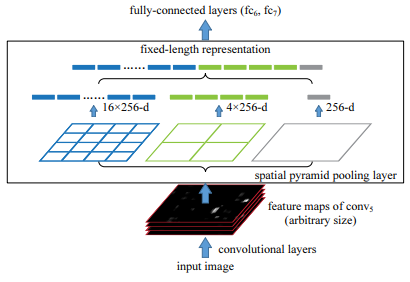
\includegraphics{spp}
\end{center}

For training and testing a model with an SPP layer several approaches can be taken. We chose to investigate a multi-size training approach, here we create two fixed-size networks that share parameters. Then for training we alternated by providing the network 32x32 images for one epoch and then 64x64 epochs for the next epoch. 

\subsubsection{Over-sampling vs Under-sampling}
\paragraph{}
Over-sampling balances a dataset by randomly duplicating the "better" representations of elements from the minority classes. However, this may cause over fitting because of the duplications. Under-sampling balances a dataset by randomly eliminating elements uniformly from the majority classes as it makes a K-means to reduce the number of samples. 

To over-sample our dataset, we used the following methods from the imbalance-learn library:

\begin{itemize}
	\item imblearn.over\_sampling.SMOTE: over-sampled on the image dataset using "not majority" for the \textit{sample\_strategy} parameter
	
	\item imblearn.over\_sampling.ADASYN: over-sampled on the image dataset using "not majority" for the \textit{sample\_strategy} parameter
	
\end{itemize}

The SMOTE algorithm applies KNN approach where it selects K nearest neighbors, joins them and creates the synthetic samples in the space. The algorithm takes the feature vectors and its nearest neighbors, computes the distance between these vectors, and multiplies it by a random number between (0, 1) and it is added back to feature. 
The ADASYN algorithm is based on the idea of adaptively generating minority data samples according to their distributions using K nearest neighbor. The algorithm adaptively updates the distribution and there are no assumptions made for the underlying distribution of the data.  The algorithm uses Euclidean distance for KNN Algorithm. 
The key difference between SMOTE and ADASYN is that the former generates the same number of synthetic samples for each of the minority classes while the latter uses a density distribution, as a criterion to automatically decide the number of synthetic samples that must be generated for each minority sample by adaptively changing the weights of the different minority samples to compensate for the skewed distributions.

\section{Results}

\begin{minipage}[c]{\textwidth}
	%%%%%%%%%%%%%%%%%%%%%%%%%
	%   resize no sampling  %
	%%%%%%%%%%%%%%%%%%%%%%%%%

\subsubsection{Resizing unbalanced dataset by scaling using nearest interpolation}

	\centering
%32x32
	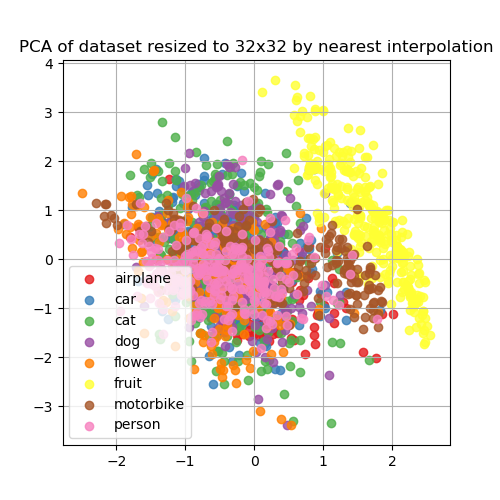
\includegraphics[width= \figureWidth\textwidth]{./figures/pca_h32_w32_r_none.png}
	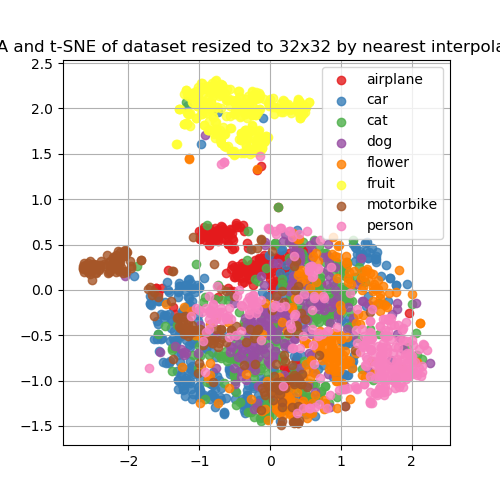
\includegraphics[width= \figureWidth\textwidth]{./figures/pca_tsne_h32_w32_r_none.png}
	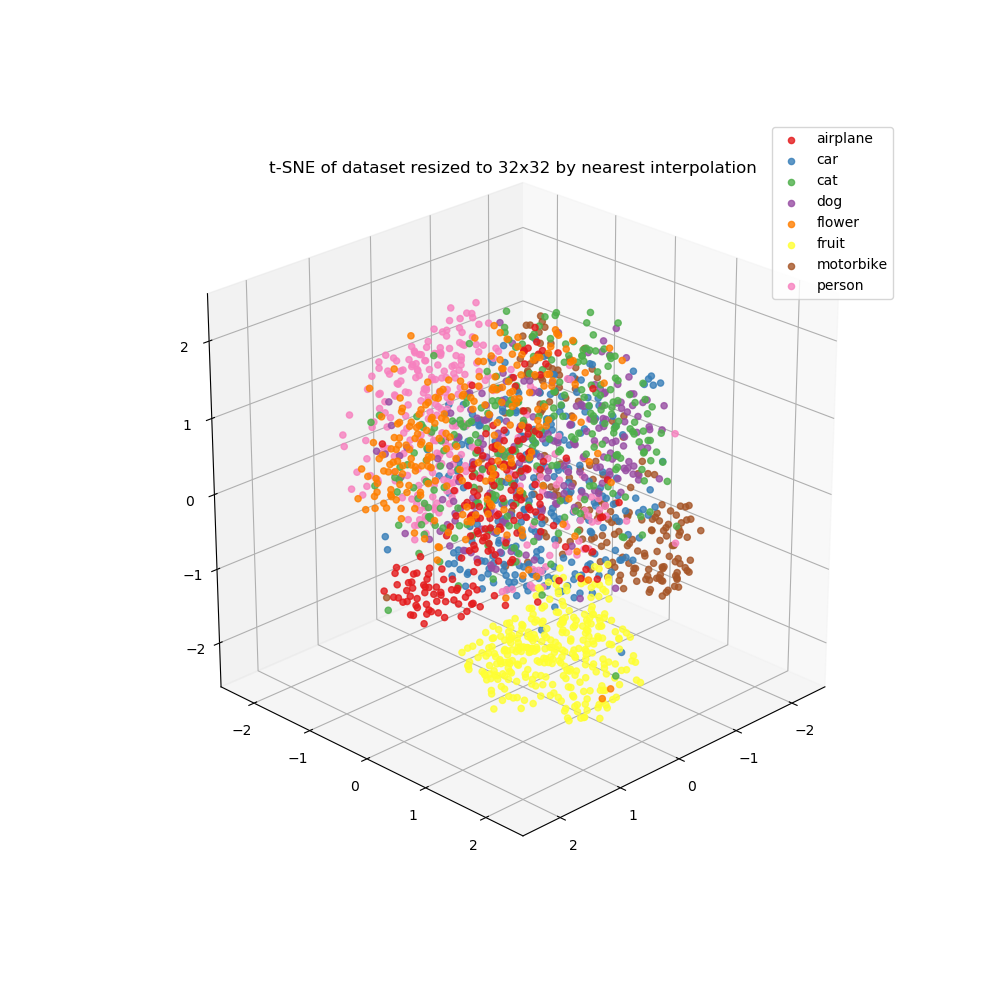
\includegraphics[width= \figureWidth\textwidth]{./figures/tsne_h32_w32_r_none.png}
	\captionof{figure}{Visualization of 2000 randomly picked data points for 32x32 rescaled images}
	
	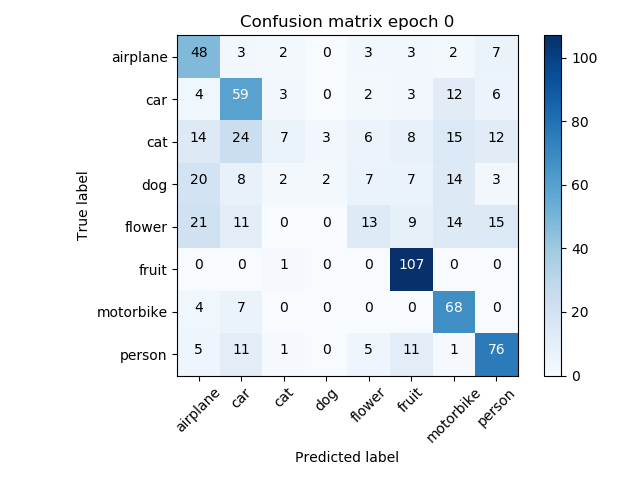
\includegraphics[width= \figureWidth\textwidth]{./figures/cm_h32_w32_r_none_e0.png}
	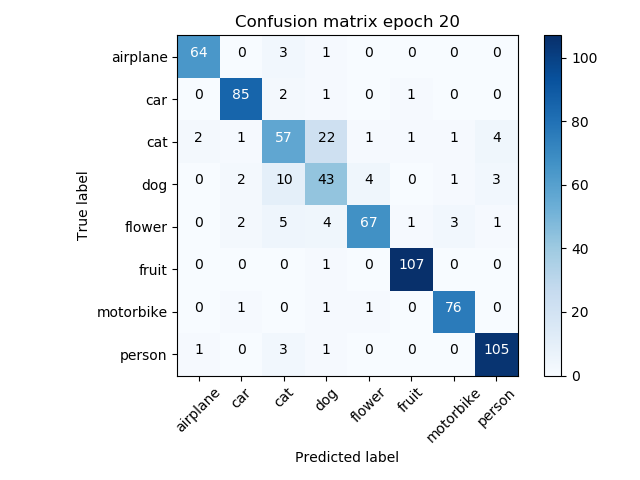
\includegraphics[width= \figureWidth\textwidth]{./figures/cm_h32_w32_r_none_e20.png}
	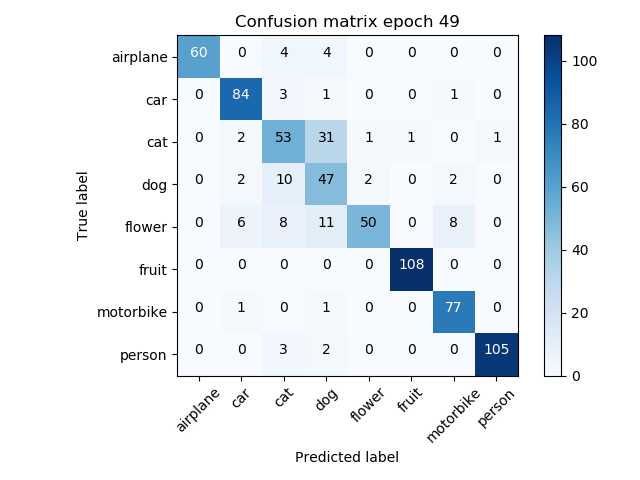
\includegraphics[width= \figureWidth\textwidth]{./figures/cm_h32_w32_r_none_e49.png}
	\captionof{figure}{Visualization of 2000 randomly picked data points for 32x32 rescaled images}
	%64x64

\end{minipage}

\begin{minipage}[c]{\textwidth}
	\centering
	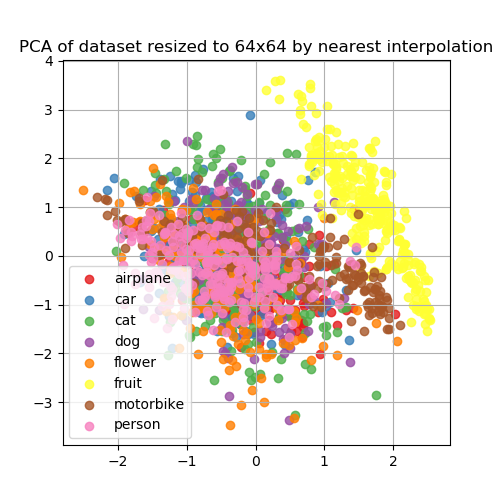
\includegraphics[width= \figureWidth\textwidth]{./figures/pca_h64_w64_r_none.png}
	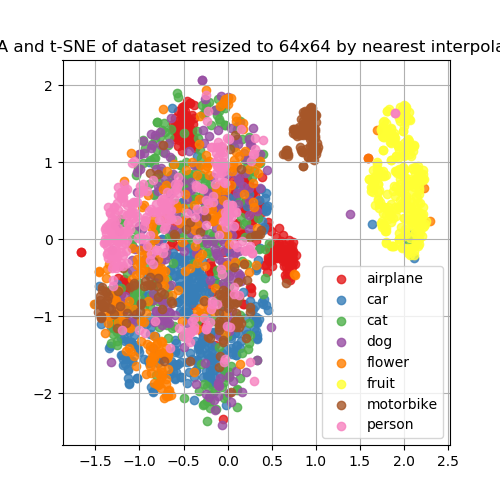
\includegraphics[width= \figureWidth\textwidth]{./figures/pca_tsne_h64_w64_r_none.png}
	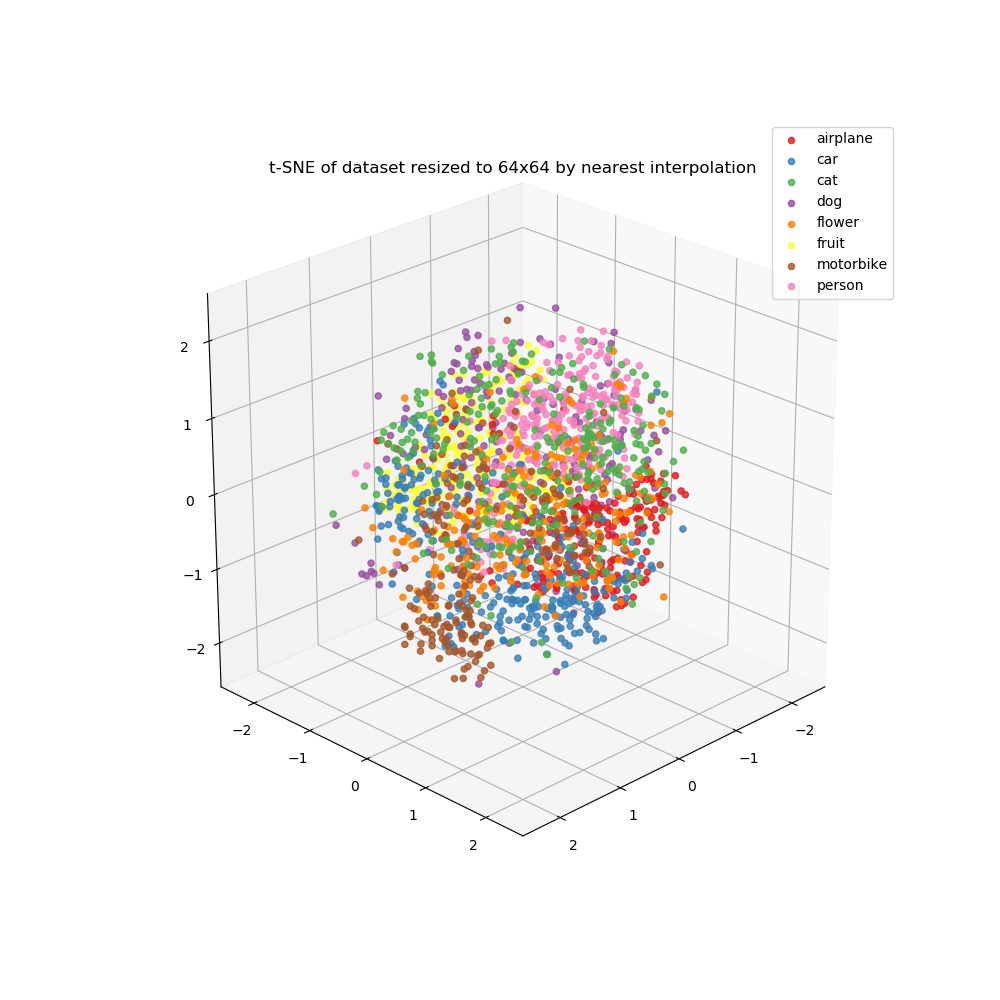
\includegraphics[width= \figureWidth\textwidth]{./figures/tsne_h64_w64_r_none.png}	\captionof{figure}{Visualization of 2000 randomly picked data points for 64x64 rescaled images}
	
	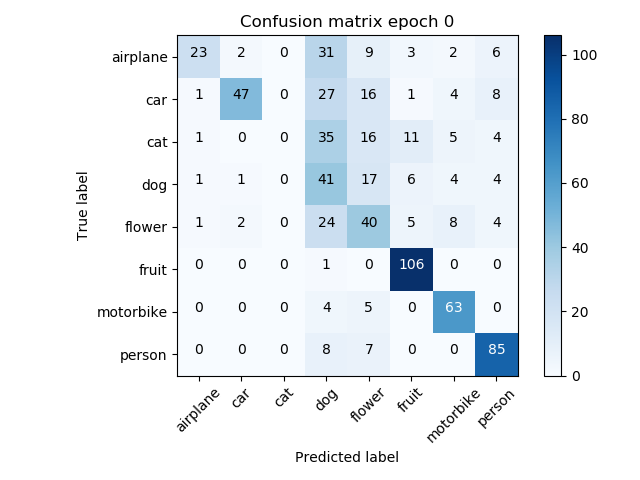
\includegraphics[width= \figureWidth\textwidth]{./figures/cm_h64_w64_r_none_e0.png}
	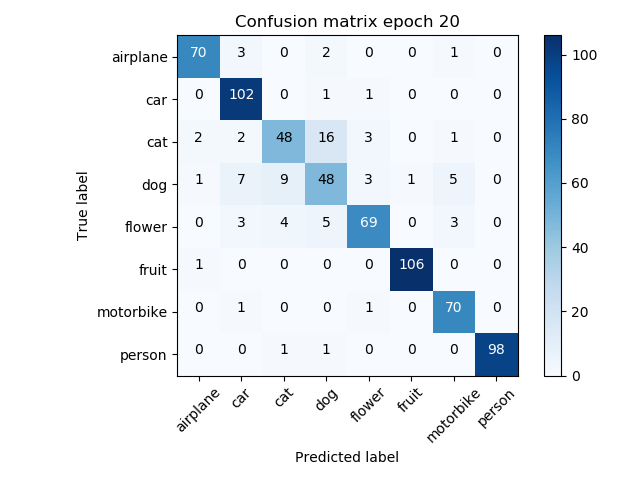
\includegraphics[width= \figureWidth\textwidth]{./figures/cm_h64_w64_r_none_e20.png}
	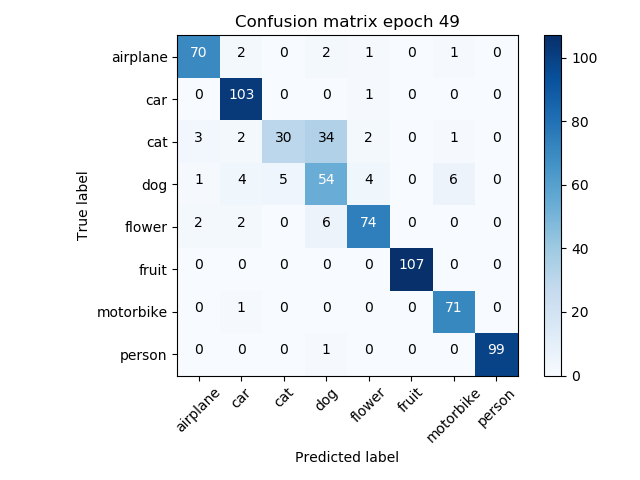
\includegraphics[width= \figureWidth\textwidth]{./figures/cm_h64_w64_r_none_e49.png}
	\captionof{figure}{Confusion Matrices of unbalanced resized images to 64x64 by scaling}
	

	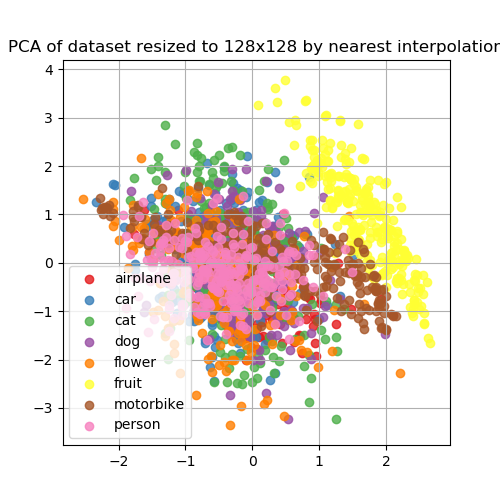
\includegraphics[width= \figureWidth\textwidth]{./figures/pca_h128_w128_r_none.png}
	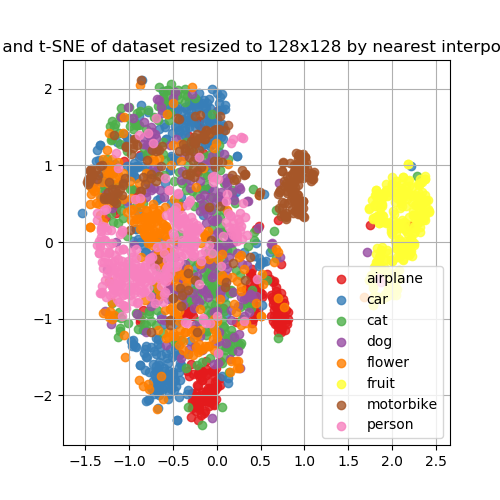
\includegraphics[width= \figureWidth\textwidth]{./figures/pca_tsne_h128_w128_r_none.png}
	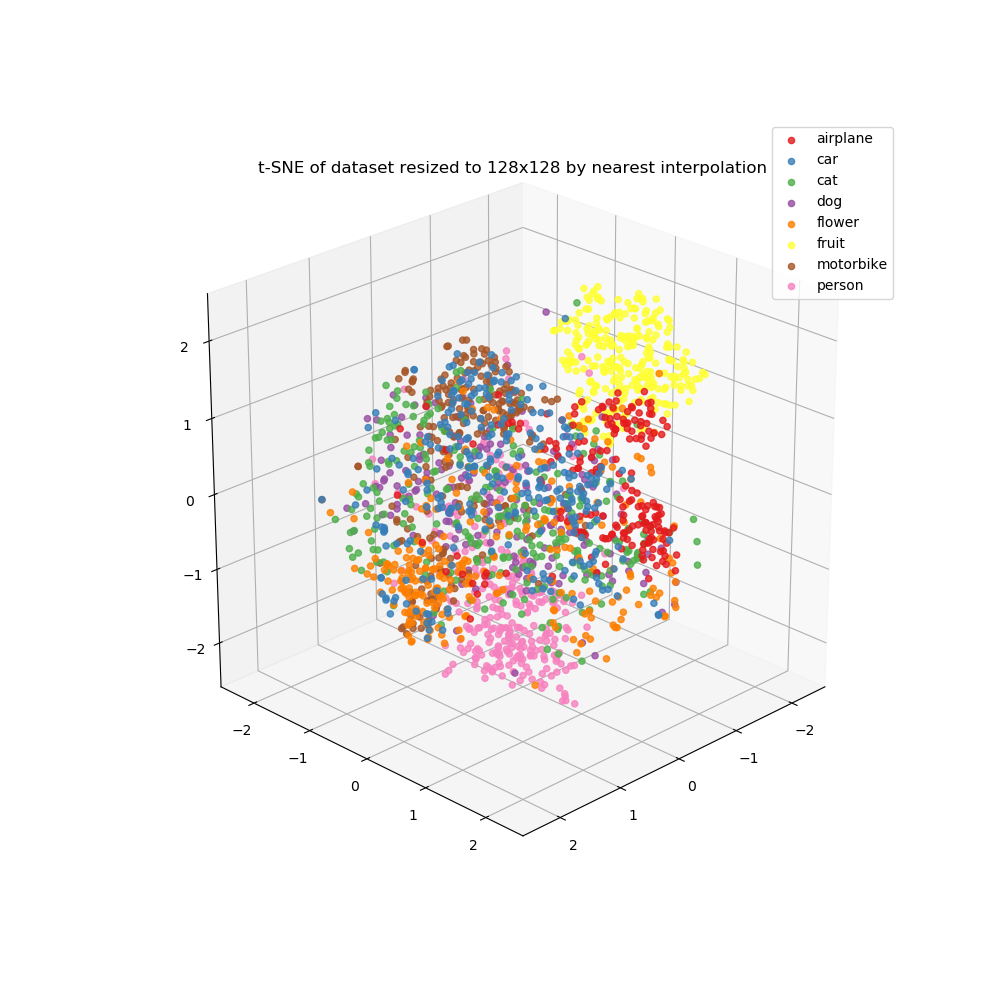
\includegraphics[width= \figureWidth\textwidth]{./figures/tsne_h128_w128_r_none.png}
	\captionof{figure}{Visualization of 2000 randomly picked data points for 128x128 rescaled images}

	\centering
	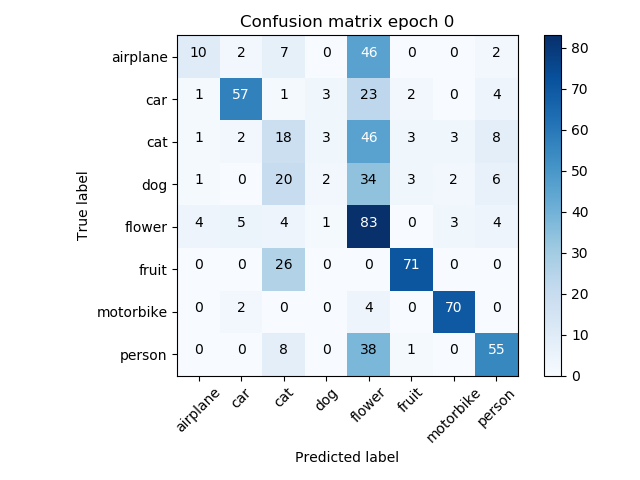
\includegraphics[width= \figureWidth\textwidth]{./figures/cm_h128_w128_r_none_e0.png}
	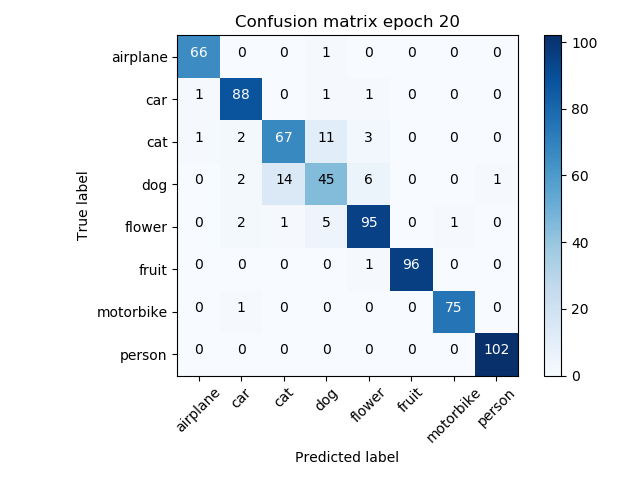
\includegraphics[width= \figureWidth\textwidth]{./figures/cm_h128_w128_r_none_e20.png}
	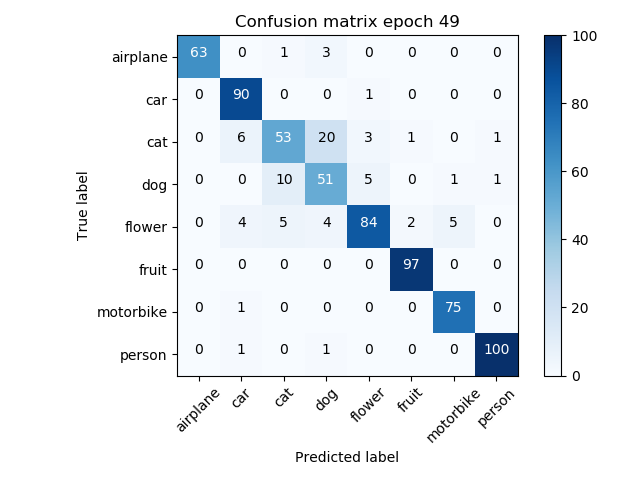
\includegraphics[width= \figureWidth\textwidth]{./figures/cm_h128_w128_r_none_e49.png}
	\captionof{figure}{Confusion Matrices of unbalanced resized images to 128x128 by scaling}
	
	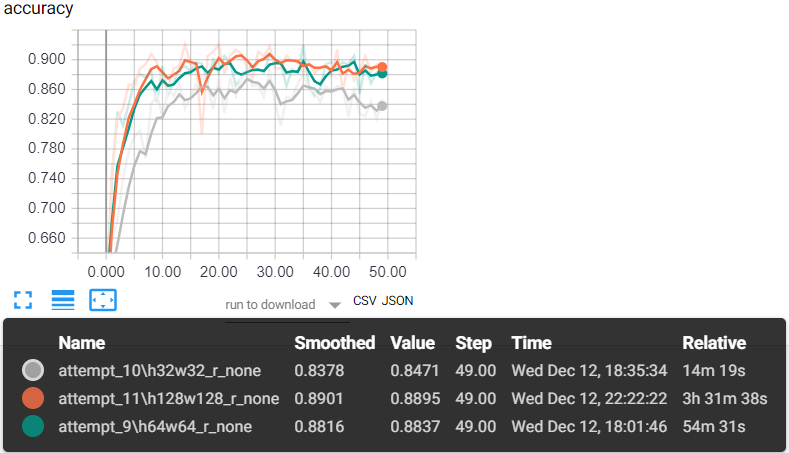
\includegraphics[width=0.5\textwidth]{./figures/acc_r_none.png}
	\captionof{figure}{Testing accuracy comparison for image scaled to 32x32 (grey), 64x64 (green), 128x128 (orange)}
\end{minipage}

%%%%%%%%%%%%%%%%%%%%%%
% CROP AND PAD
\begin{minipage}[c]{\linewidth}
	\subsubsection{Resizing unbalanced dataset by crop and pad}
	\centering
	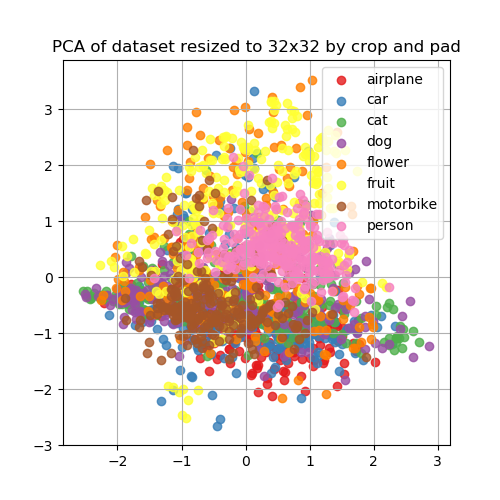
\includegraphics[width= \figureWidth\textwidth]{./figures/pca_h32_w32_cp_none.png}
	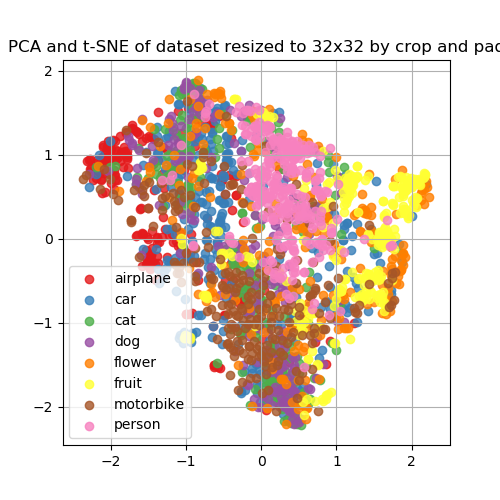
\includegraphics[width= \figureWidth\textwidth]{./figures/pca_tsne_h32_w32_cp_none.png}
	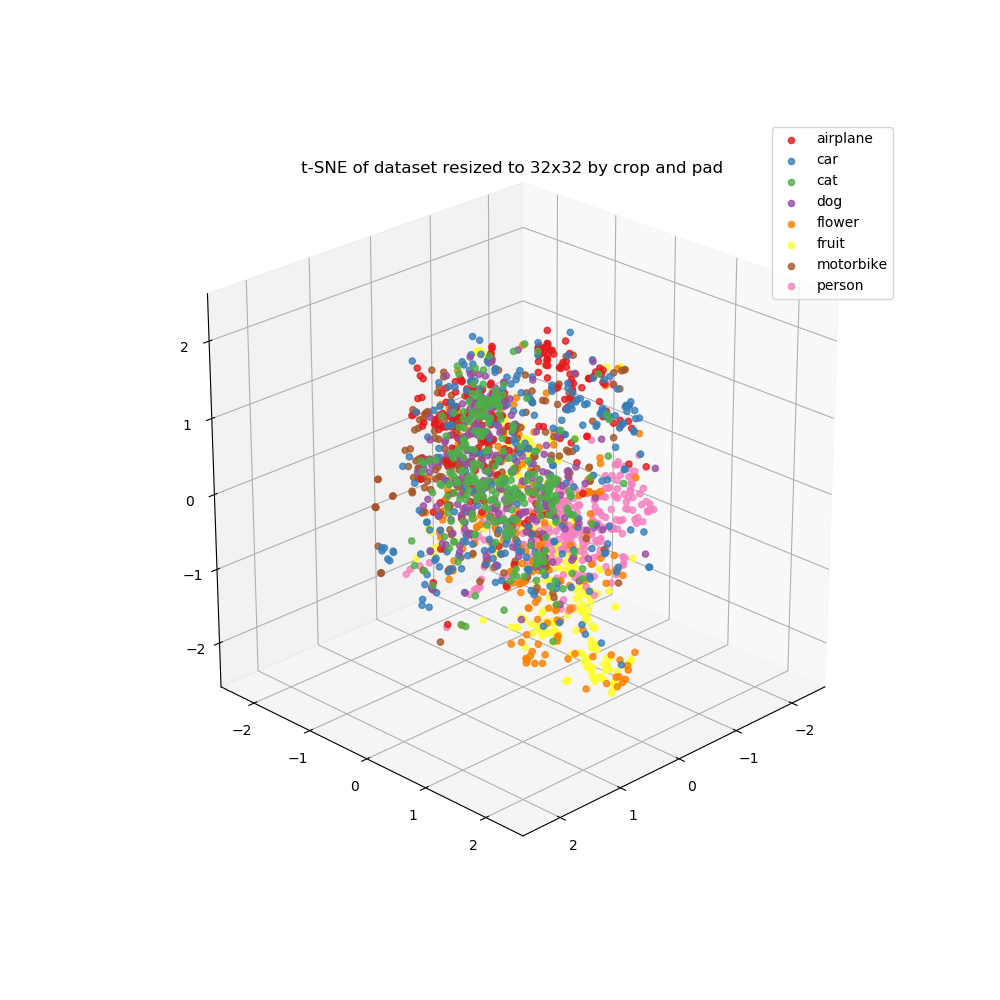
\includegraphics[width= \figureWidth\textwidth]{./figures/tsne_h32_w32_cp_none.png}
	\captionof{figure}{Visualization of 2000 randomly picked data points for 32x32 crop/pad images}
	
	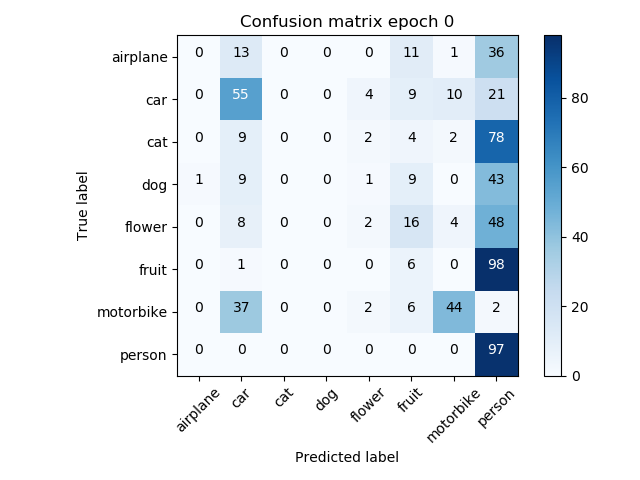
\includegraphics[width=\figureWidth\textwidth]{./figures/cm_h32_w32_cp_none_e0.png}
	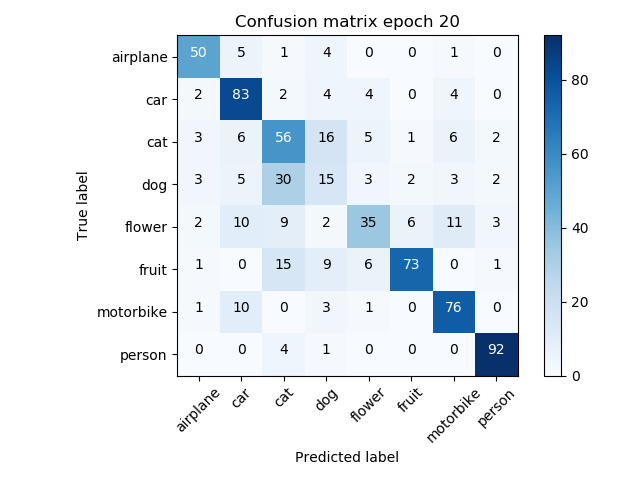
\includegraphics[width= \figureWidth\textwidth]{./figures/cm_h32_w32_cp_none_e20.png}
	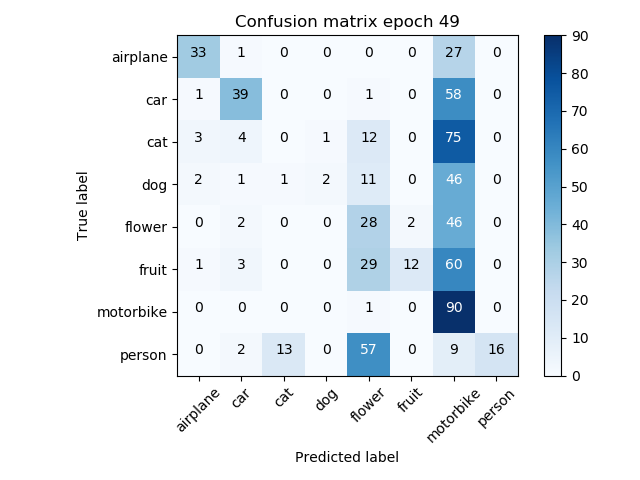
\includegraphics[width= \figureWidth\textwidth]{./figures/cm_h32_w32_cp_none_e49.png}
	\captionof{figure}{Confusion Matrices of unbalanced resized images to 32x32 by crop/pad}	
	
	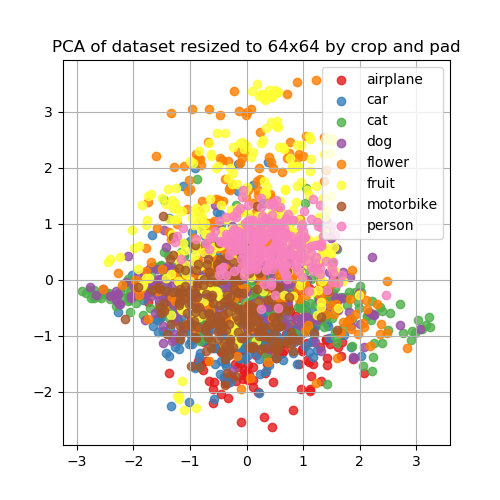
\includegraphics[width= \figureWidth\textwidth]{./figures/pca_h64_w64_cp_none.png}
	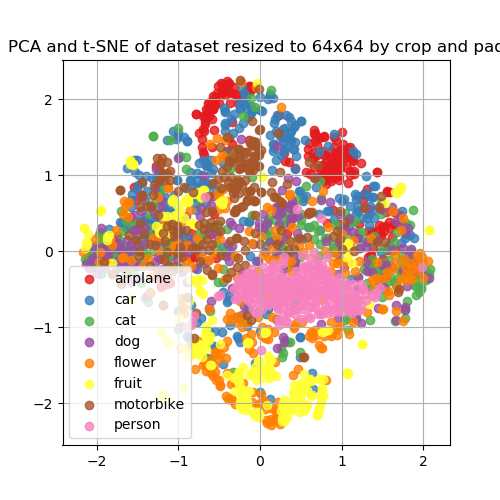
\includegraphics[width= \figureWidth\textwidth]{./figures/pca_tsne_h64_w64_cp_none.png}
	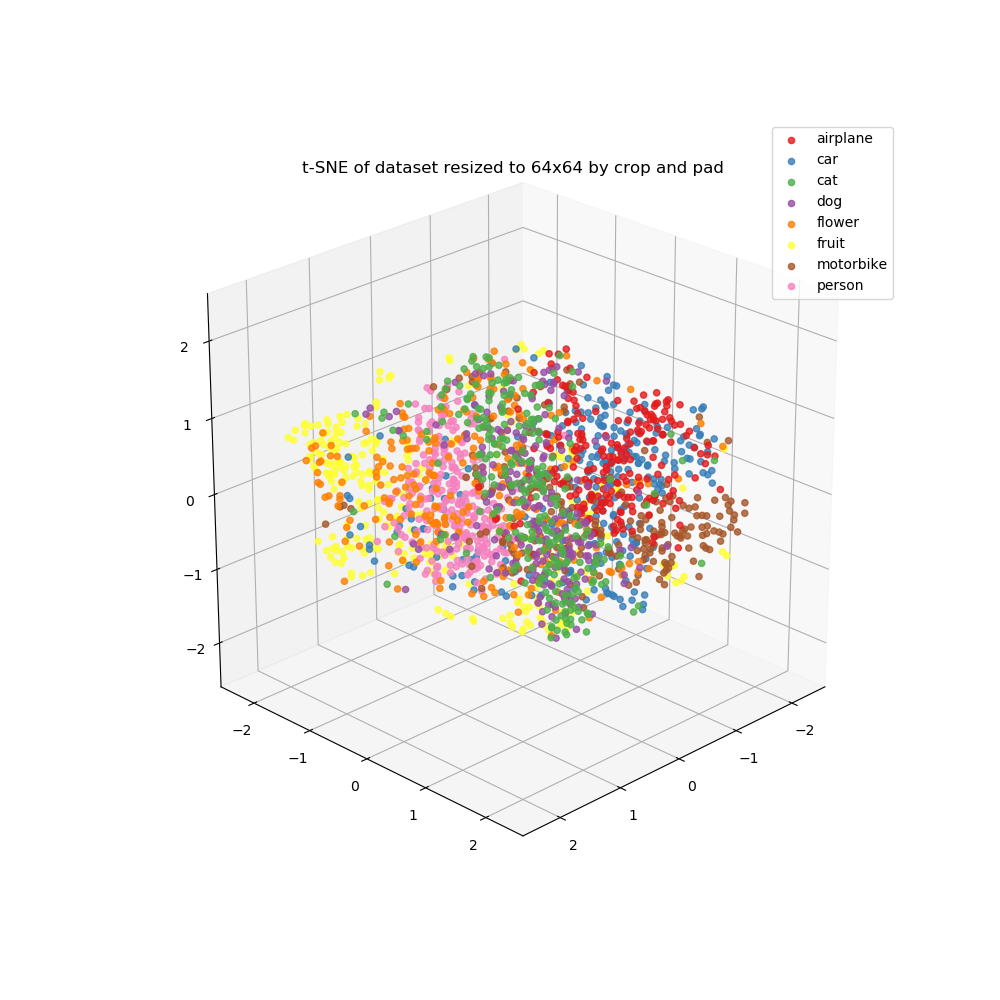
\includegraphics[width= \figureWidth\textwidth]{./figures/tsne_h64_w64_cp_none.png}
	\captionof{figure}{Visualization of 2000 randomly picked data points for 64x64 crop/pad images}
	
	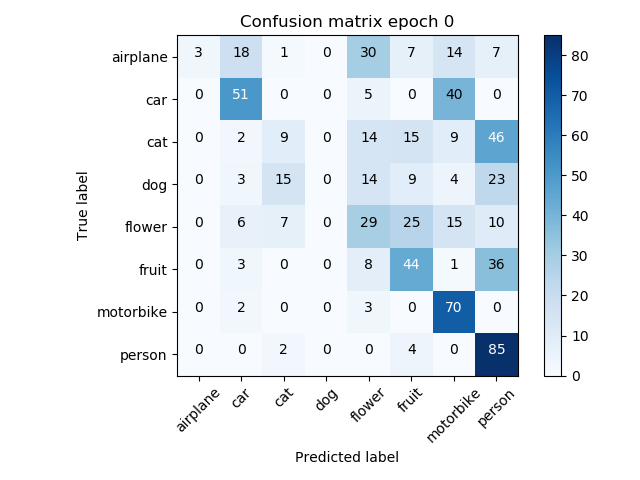
\includegraphics[width=\figureWidth\textwidth]{./figures/cm_h64_w64_cp_none_e0.png}
	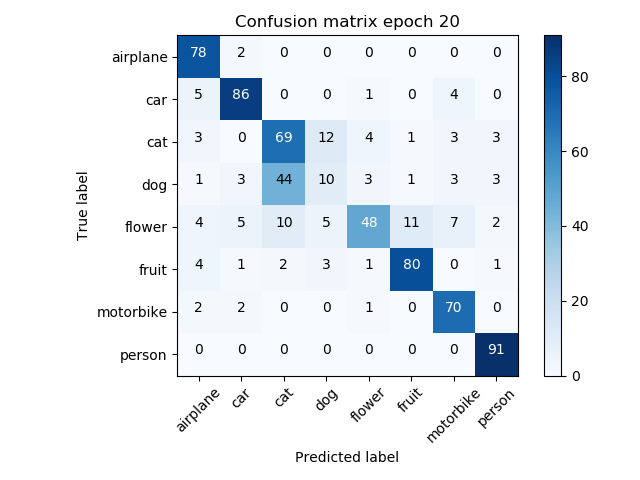
\includegraphics[width= \figureWidth\textwidth]{./figures/cm_h64_w64_cp_none_e20.png}
	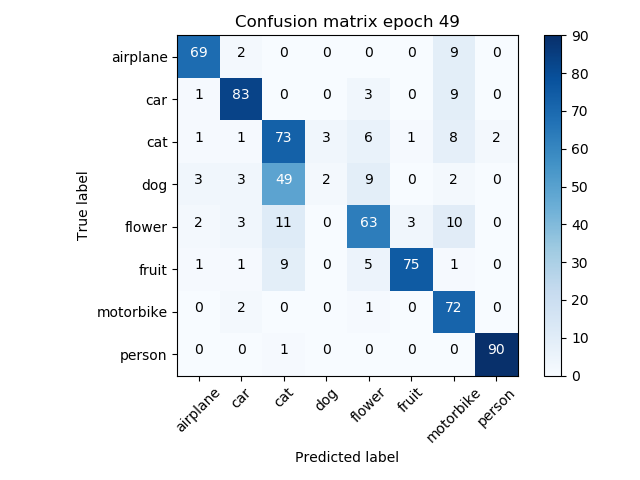
\includegraphics[width= \figureWidth\textwidth]{./figures/cm_h64_w64_cp_none_e49.png}
	\captionof{figure}{Confusion Matrices of unbalanced resized images to 64x64 by crop/pad}

	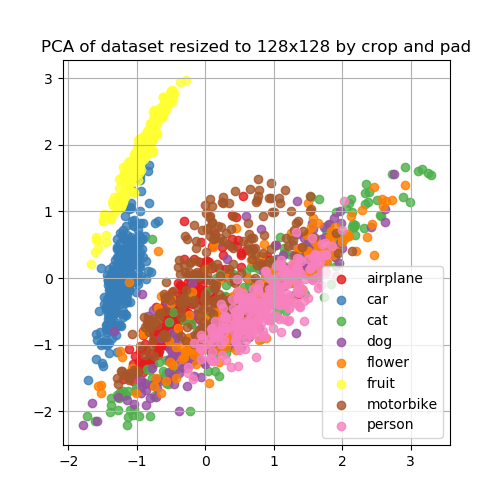
\includegraphics[width= \figureWidth\textwidth]{./figures/pca_h128_w128_cp_none.png}
	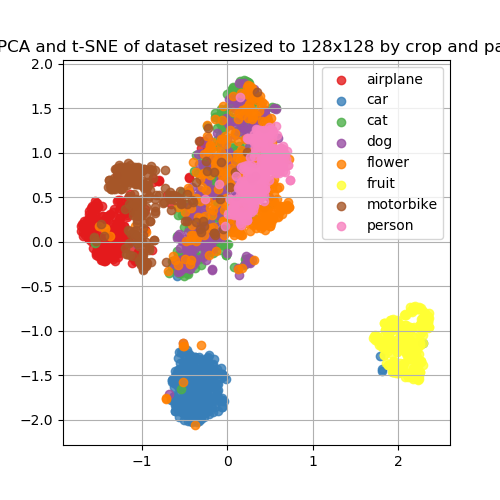
\includegraphics[width= \figureWidth\textwidth]{./figures/pca_tsne_h128_w128_cp_none.png}
	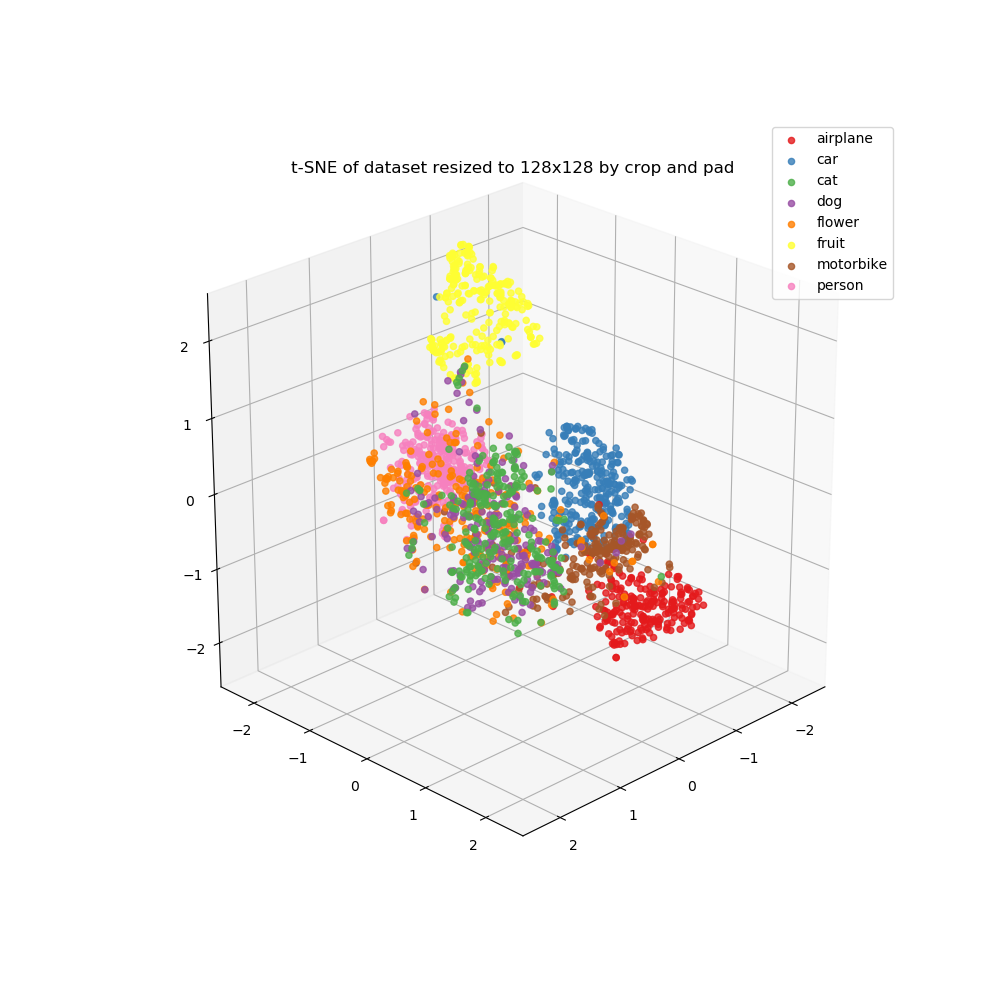
\includegraphics[width= \figureWidth\textwidth]{./figures/tsne_h128_w128_cp_none.png}
	\captionof{figure}{Visualization of 2000 randomly picked data points for 128x128 crop/pad images}
\end{minipage}

\begin{minipage}[c]{\linewidth}
    \centering
	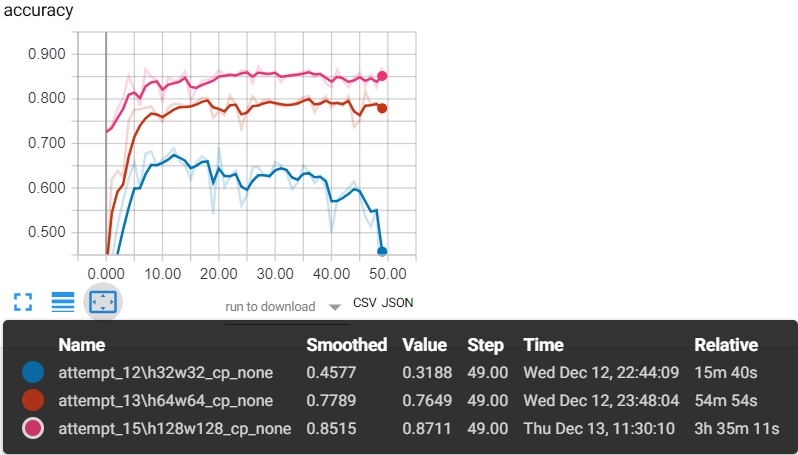
\includegraphics[width=0.5\textwidth]{./figures/acc_cp_none.png}
	\captionof{figure}{Testing accuracy comparison for image resized by nearest interpolation for 32x32 (blue), 64x64 (red), 128x128 (pink)}
	
	' '\\
	\raggedright
	\subsubsection{Up-sampling dataset using SMOTE and ADASYN on 64x64 rescaled images}
	
	\centering
	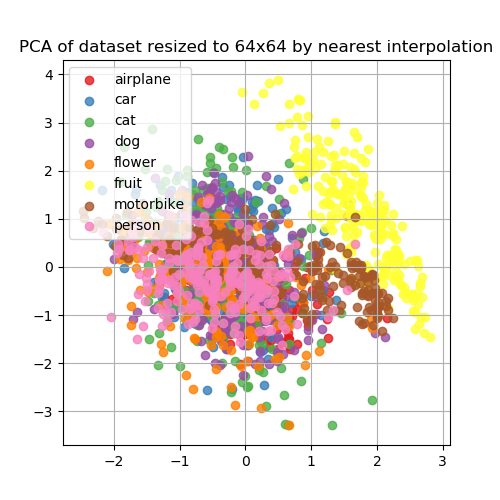
\includegraphics[width=\figureWidth\textwidth]{./figures/pca_h64_w64_r_smote.png}
	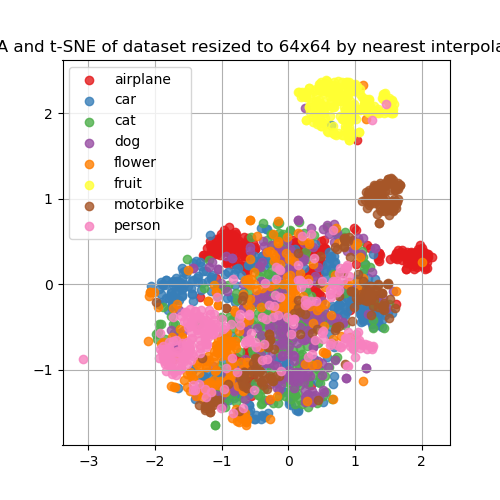
\includegraphics[width=\figureWidth\textwidth]{./figures/pca_tsne_h64_w64_r_smote.png}
	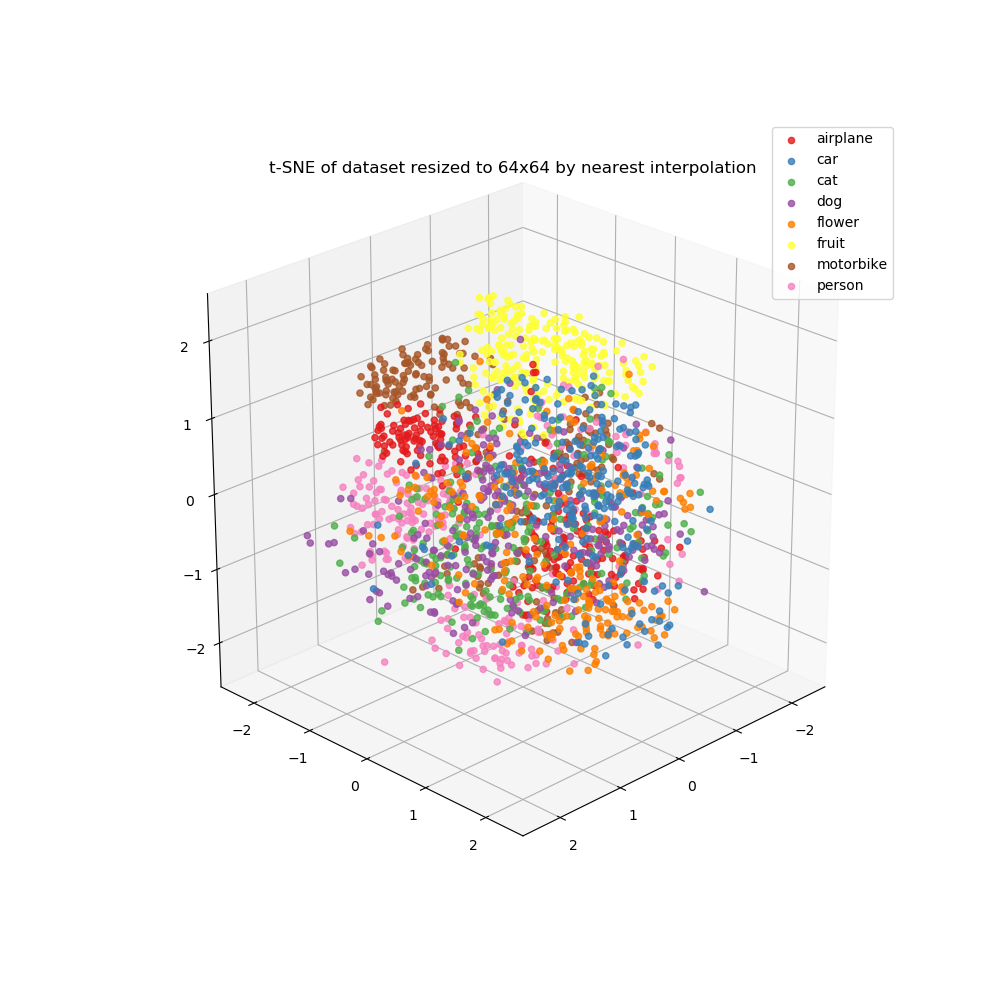
\includegraphics[width=\figureWidth\textwidth]{./figures/tsne_h64_w64_r_smote.png}
	\captionof{figure}{Visualization of 2000 randomly picked up-sampled data points by SMOTE for 64x64 images resized by nearest interpolation}
	
	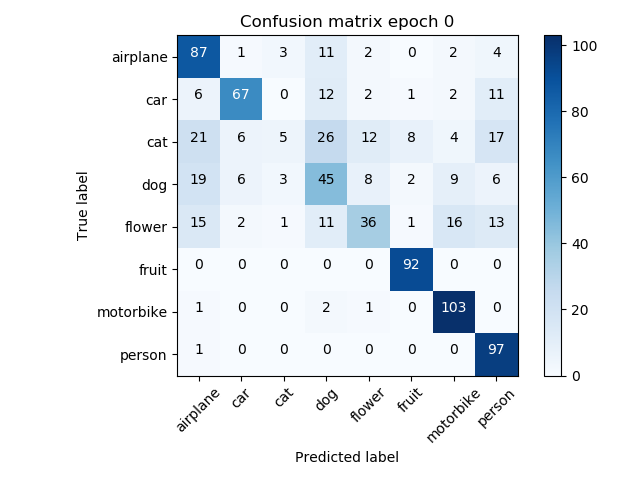
\includegraphics[width=\figureWidth\textwidth]{./figures/cm_h64_w64_r_smote_e0.png}
	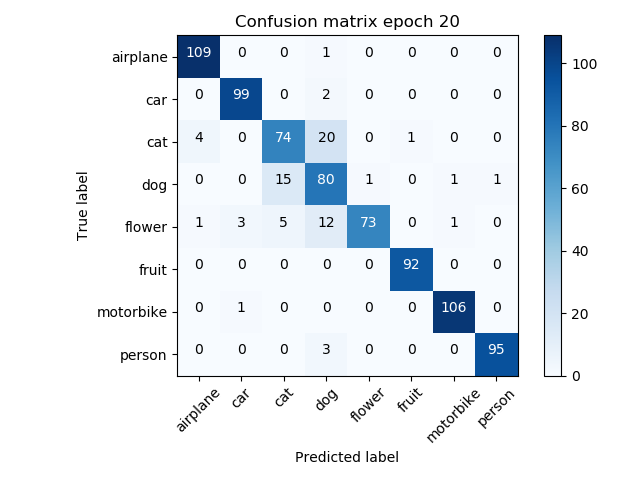
\includegraphics[width=\figureWidth\textwidth]{./figures/cm_h64_w64_r_smote_e20.png}
	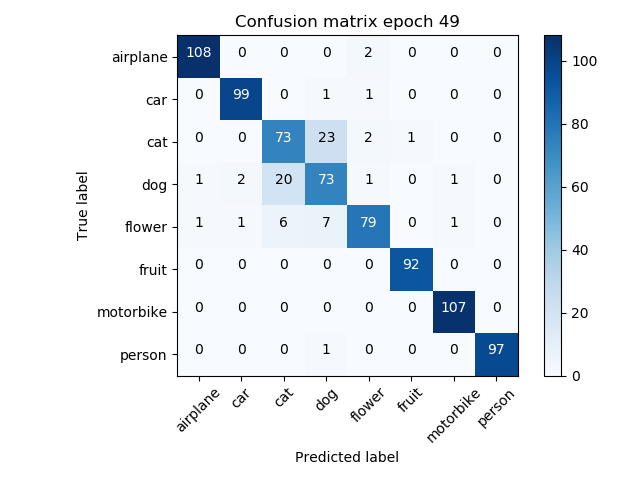
\includegraphics[width=\figureWidth\textwidth]{./figures/cm_h64_w64_r_smote_e49.png}
	\captionof{figure}{Confusion matrix up-sampled data points by SMOTE for 64x64 images resized by nearest interpolation}
	
	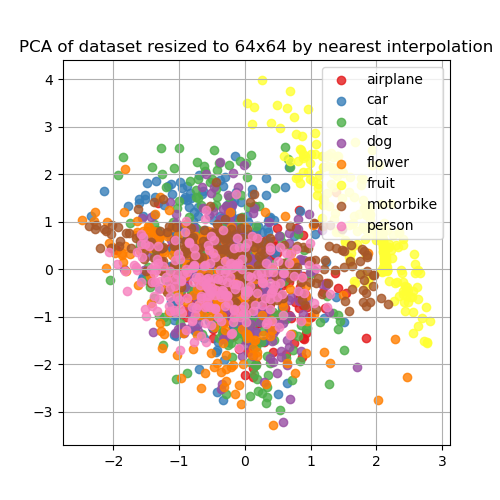
\includegraphics[width=\figureWidth\textwidth]{./figures/pca_h64_w64_r_adasyn.png}
	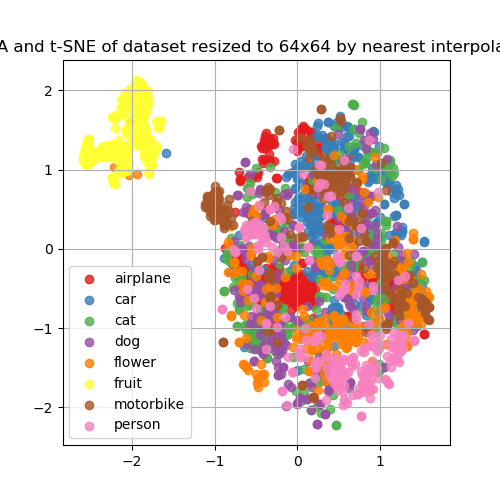
\includegraphics[width=\figureWidth\textwidth]{./figures/pca_tsne_h64_w64_r_adasyn.png}
	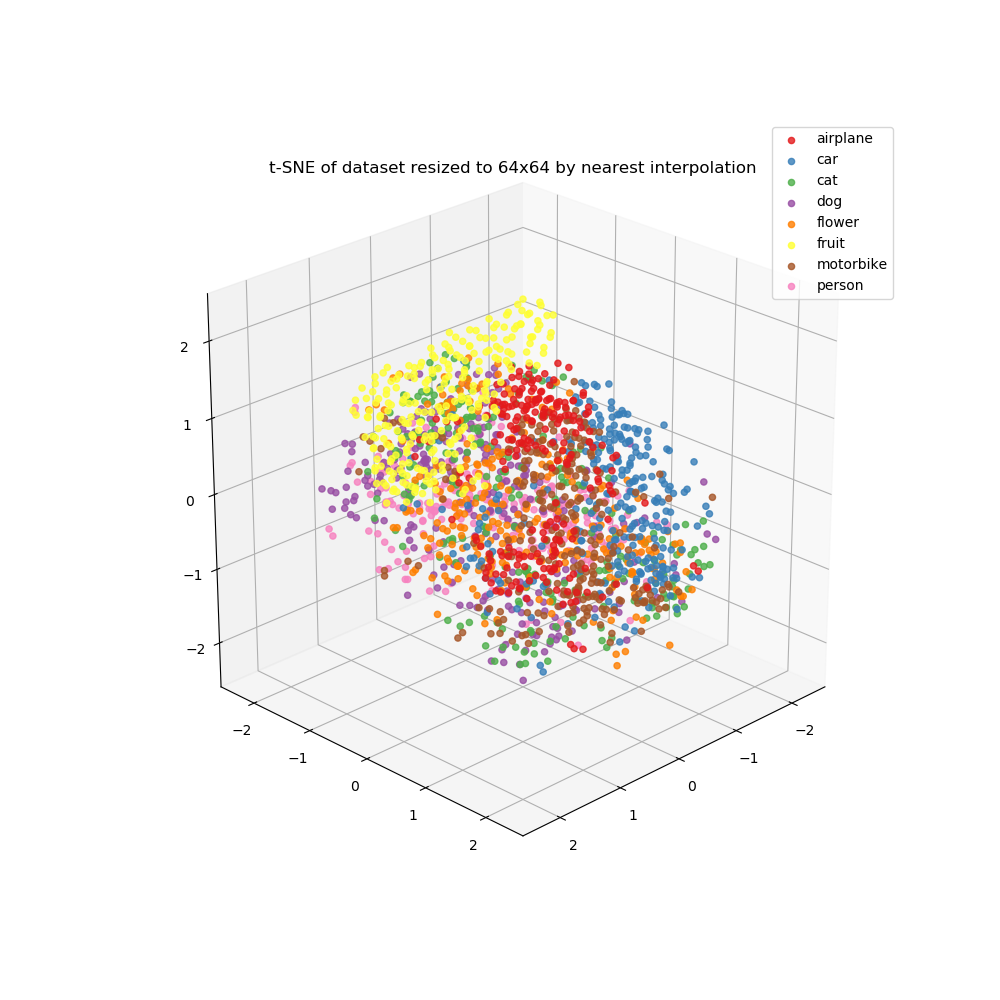
\includegraphics[width=\figureWidth\textwidth]{./figures/tsne_h64_w64_r_adasyn.png}
	\captionof{figure}{Visualization of 2000 randomly picked up-sampled data points by ADASYN for 64x64 images resized by nearest interpolation}
	
\end{minipage}

\begin{minipage}[c]{\linewidth}
	\centering
	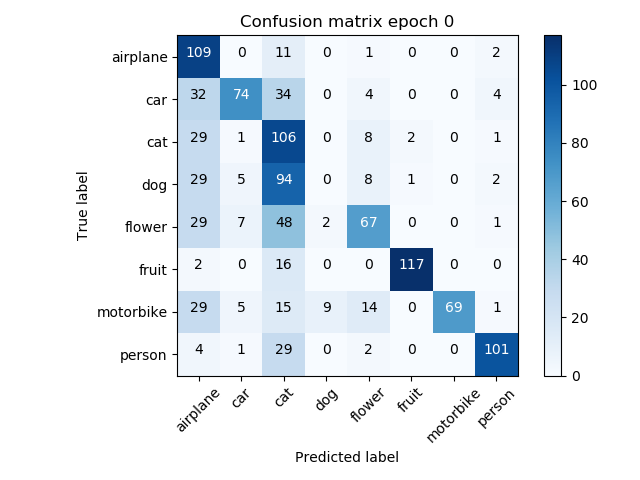
\includegraphics[width=\figureWidth\textwidth]{./figures/cm_h64_w64_r_adasyn_e0.png}
	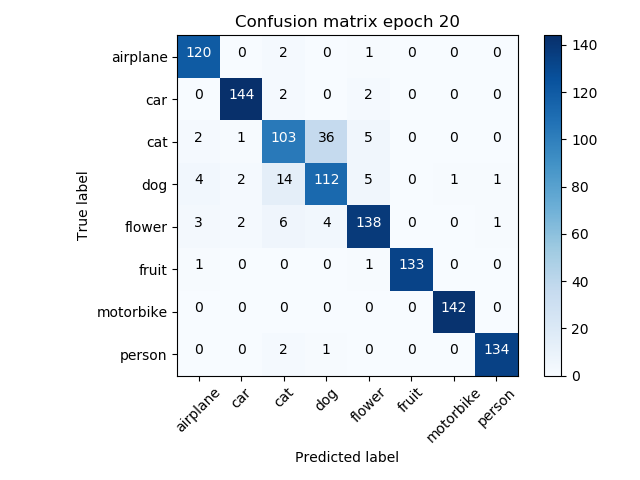
\includegraphics[width=\figureWidth\textwidth]{./figures/cm_h64_w64_r_adasyn_e20.png}
	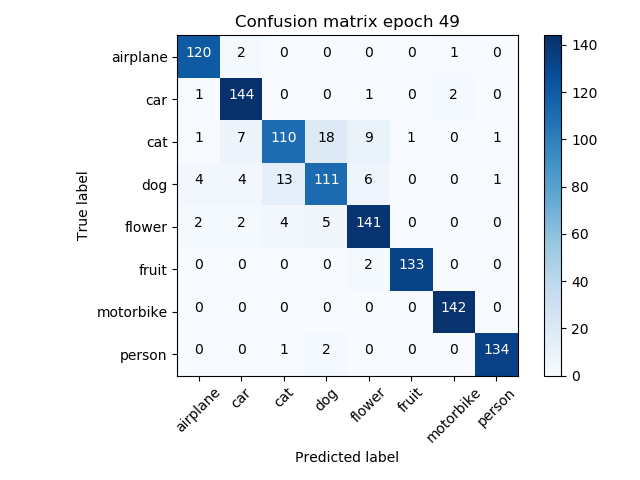
\includegraphics[width=\figureWidth\textwidth]{./figures/cm_h64_w64_r_adasyn_e49.png}
	\captionof{figure}{Visualization of 2000 randomly picked up-sampled data points by ADASYN for 64x64 images resized by nearest interpolation}
	
	
	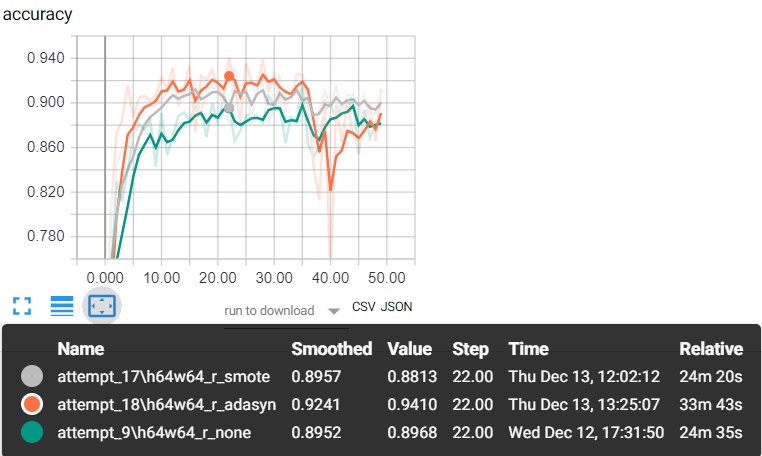
\includegraphics[width=0.5\textwidth]{./figures/acc_smote_adaysn_none.png}
	\captionof{figure}{Testing accuracy comparison between no-upsampling (green), SMOTE (grey) and ADASYN (orange) on 64x64 image dataset}
	
\end{minipage}


\section{Analysis and Discussion}
\paragraph{}
We compared results between resizing by scaling and crop and pad. Each experiment ran for 50 epochs and the resulting accuracies were tabulated as shown below:

\begin{table}[ht]
	\caption{Accuracy Comparison of Scaled vs Crop and Pad} % title of Table
	\centering % used for centering table
	\begin{tabular}{c c c c c c c c} % centered columns (4 columns)
		\hline\hline %inserts double horizontal lines
		
		Epoch &  \multicolumn{3}{c}{Scale} & \multicolumn{3}{c}{Crop and Pad}\\
		\hline
		
		{} & 32x32 & 64x64 & 128x128 & 32x32 & 64x64 & 128x128 \\ [0.5ex] % inserts table
		%heading
		\hline % inserts single horizontal line
		5 & 79.79 & 87.12 & 86.51 & 65.87 & 77.59 & 82.03\\
		10 & 82.82 & 89.10 & 87.02 & 66.49 & 75.01 & 84.83\\
		20 & 87.42 & 90.52 & 92.06 & 69.18 & 80.70 & 86.41\\
		50 & 84.71& 88.37 & 88.95 & 55.14 & 76.49 & 87.11\\ [1ex] % [1ex] adds vertical space
		\hline %inserts single line
	\end{tabular}
	\label{table:scale_cp} % is used to refer this table in the text
\end{table}
In general, the training seems to have converged at approximately 20 epochs before over fitting as we can see that at 50 epochs the accuracy is worse than at 20 epochs. 
The results from the different resizing techniques show that in general, resizing by scaling the image is significantly better than cropping and padding, as can be seen from Figure 6 and Figure 13 and Table 1. We note that each size increment for cropping and padding an image results in a significant accuracy increase and this is reasonable because of the nature of how crop and pad processes an image. When an image is resized by crop and pad, we either directly crop out the extra rows and columns of pixels if it is too large, or pad them with black pixels. The idea is to retain the image resolution and not skew it. However, if the original image is much larger than the resulting size, we directly remove a large amount of data which will cause poor performance. For example, if we resize a cat image of 64x64 to a 32x32 image by cropping it, the resulting image will only hold the center chest area of the cat, thus losing the "arm", "leg" and "head" features of a cat. Conversely, resizing an image by scaling it with nearest interpolation is a much better approach at reducing noise because each image still holds the full picture. This also explains why the images scaled to 32x32 does just as well as an image that is cropped and padded to 128x128. However, we have not tried a large enough size in which cropping was unnecessary and the images would only be padded with black pixels. It may be interesting to observe the performance for images that are only padded because then no information is lost. Then, we would be comparing the performance for adding black pixel as noise versus stretching an image to a specified size. 

We then investigated the Imbalance Class problem by comparing performance results on imbalanced dataset and balanced datset of 64x64 re-scaled images. The accuracy results of each experiment were tabulated as shown below:
\begin{table}[ht]
	\caption{Accuracy Comparison of None, SMOTE and ADASYN on 64x64 dataset} % title of Table
	\centering % used for centering table
	\begin{tabular}{c c c c} % centered columns (4 columns)
		\hline\hline %inserts double horizontal lines
		
		Epoch &  None & SMOTE & ADASYN\\
		\hline

		\hline % inserts single horizontal line
		5  &  87.12 & 86.87 & 88.77\\
		10 &  89.10 & 90.25 & 90.71\\
		20 &  90.52 & 93.00 & 94.10\\
		50 &  88.37 & 89.67 & 91.25\\ [1ex] % [1ex] adds vertical space
		\hline %inserts single line
	\end{tabular}
	\label{table:balanced} % is used to refer this table in the text
\end{table} 

The results show that balancing a data does indeed improve the overall performance, but since we only performed 1-fold, the results may not be an accurate representation. Despite balancing the dataset, the network is still incapable of differentiating dogs and cats with certainty. We can observe this by looking at the confusion matrices on Figure 4, Figure 15 and Figure 17. Looking at the middle matrix for each figure, we see that the ratio of misidentifying cats and dogs are approximately the same and this is because the up-sampling technique only duplicates our data and cannot reproduce new cat and dog images that hold distinctive traits. 

\section{Conclusion	}
\paragraph{}
In conclusion, different resizing techniques can make a significant different to classification accuracy, and balanced datasets do improve classification accuracy. From our experiments, scaling an image is generally a better approach as it retains the most information. Balanced datasets also improve the overall performance of the neural network. 
\section{References	}
https://www.datasciencecentral.com/profiles/blogs/handling-imbalanced-data-sets-in-supervised-learning-using-family

\end{document} 